%%%%%%%%%%%%%%%%%%%%%%%%%%%%%%%%%%%%%%%%%
% Short Sectioned Assignment
% LaTeX Template
% Version 1.0 (5/5/12)
%
% This template has been downloaded from:
% http://www.LaTeXTemplates.com
%
% Original author:
% Frits Wenneker (http://www.howtotex.com)
%
% License:
% CC BY-NC-SA 3.0 (http://creativecommons.org/licenses/by-nc-sa/3.0/)
%
%%%%%%%%%%%%%%%%%%%%%%%%%%%%%%%%%%%%%%%%%

%----------------------------------------------------------------------------------------
%	PACKAGES AND OTHER DOCUMENT CONFIGURATIONS
%----------------------------------------------------------------------------------------

\documentclass[paper=a4, fontsize=11pt]{scrartcl} % A4 paper and 11pt font size

\usepackage{graphicx}
\graphicspath{ {images/} }
\usepackage{verbatim}
\usepackage{textcomp}
\usepackage{changepage}
\usepackage[T1]{fontenc} % Use 8-bit encoding that has 256 glyphs
\usepackage{fourier} % Use the Adobe Utopia font for the document - comment this line to return to the LaTeX default
\usepackage[english]{babel} % English language/hyphenation
\usepackage{amsmath,amsfonts,amsthm} % Math packages

\usepackage{setspace}
\renewcommand{\baselinestretch}{1.3}
\usepackage{lipsum} % Used for inserting dummy 'Lorem ipsum' text into the template

\usepackage{color}

%\usepackage{biblatex}
%\addbibresource{sample.bib}

\usepackage{sectsty} % Allows customizing section commands
\allsectionsfont{\centering \normalfont\scshape} % Make all sections centered, the default font and small caps

\usepackage{fancyhdr} % Custom headers and footers
\pagestyle{fancyplain} % Makes all pages in the document conform to the custom headers and footers
\fancyhead{} % No page header - if you want one, create it in the same way as the footers below
\fancyfoot[L]{} % Empty left footer
\fancyfoot[C]{} % Empty center footer
\fancyfoot[R]{\thepage} % Page numbering for right footer
\renewcommand{\headrulewidth}{0pt} % Remove header underlines
\renewcommand{\footrulewidth}{0pt} % Remove footer underlines
\setlength{\headheight}{13.6pt} % Customize the height of the header

\numberwithin{equation}{section} % Number equations within sections (i.e. 1.1, 1.2, 2.1, 2.2 instead of 1, 2, 3, 4)
\numberwithin{figure}{section} % Number figures within sections (i.e. 1.1, 1.2, 2.1, 2.2 instead of 1, 2, 3, 4)
\numberwithin{table}{section} % Number tables within sections (i.e. 1.1, 1.2, 2.1, 2.2 instead of 1, 2, 3, 4)

\setlength\parindent{0pt} % Removes all indentation from paragraphs - comment this line for an assignment with lots of text

%----------------------------------------------------------------------------------------
%	TITLE SECTION
%----------------------------------------------------------------------------------------

\newcommand{\horrule}[1]{\rule{\linewidth}{#1}} % Create horizontal rule command with 1 argument of height

\title{	
\normalfont \normalsize 
\textsc{TRINITY COLLEGE DUBLIN, school of Mathematics} \\ [25pt] % Your university, school and/or department name(s)
\horrule{0.5pt} \\[0.4cm] % Thin top horizontal rule
\huge 5691 Seminar Report \\ Multiple Kernel Learning \\ % The assignment title
\horrule{2pt} \\[0.5cm] % Thick bottom horizontal rule
}

\author{Gustavo Ramirez} % Your name

\date{\normalsize\today} % Today's date or a custom date

\begin{document}

\maketitle % Print the title

%----------------------------------------------------------------------------------------
%	PROBLEM 1
%----------------------------------------------------------------------------------------

\begin{comment}
\section{Problem description}

\begin{enumerate}
\item 
\item 
\item 
\item 
\end{enumerate}

\end{comment}

\newpage


\begin{comment}

USEFUL LINKS:

official sources for terminology:
-----
http://www.intel.com/content/www/us/en/support/topics/glossary.html
https://www-01.ibm.com/software/globalization/terminology/a.html
-----




about IMB processors:
-----

insert in google: list of ibm processors
https://en.wikipedia.org/wiki/List_of_IBM_products
https://www-01.ibm.com/software/passportadvantage/guide_to_identifying_processor_family.html
http://www.nextplatform.com/2015/08/10/ibm-roadmap-extends-power-chips-to-2020-and-beyond/
http://www.theverge.com/2015/7/9/8919091/ibm-7nm-transistor-processor
https://www.ibm.com/developerworks/ibmi/library/i-ibmi-7_2-and-ibm-power8/
-----




\end{comment}


%INTRO
\section{Introduction: Machine Learning}

Machine Learning is a lot of things, and the field is constantly expanding. The boundaries of it are constantly expanding/changing. But it can be almost defined (although, it depends very much on the context). Like Arthur Lee Samuel said:

\begin{center}
\textit{[Machine Learning is the] field of study that gives computers the ability to learn without being explicitly programmed}
\end{center}

From the previous quote, it is obvious that the development and implementation of Machine Learning is a first step towards Artifial Intelligence. On the other hand (and in a less general way), Tom Mitchell (Carnegie Melon University) said:

\begin{center}
\textit{A computer program is said to learn from experience E with respect to some task T and some performance measure P, if its performance on T, as measured by P, improves with experience E}
\end{center}

To understand the previous quote more explicitly, think of fitting data using a straight line: the experience E can be the data used in obtaining the two parameters for the straight line, the performance P can be the correlation $r$, and the idea is that Machine Learning (simple linear regression in this very specific example) is useful if the correlation improves when that straight line is used again with another set of data (the task T, of course, is the prediction of results in the specific problem to be implemented).

Two major problems (see \cite{bishop1}) that Machine Learning solves are: regression and classification. The tool presented here (Multiple Kernel Learning) is useful for an algorithm solving any of those two. The \textit{regression} problem is basically a fitting problem, and the \textit{classification} is characteristic of systems where we seek a yes-or-no prediction (e.g. in a group of cells, which are useful and which aren't, for some specific task).

For a better understanding of what Machine Learning really is, it is important to compare it with other branches of data science; figure \ref{fig:ML_comparison_image} (taken from \cite{polly1}) accomplishes this. From that figure, it is interesting and important to note that \textit{Databases} has no overlap with Machine Learning.


\begin{figure}[t]
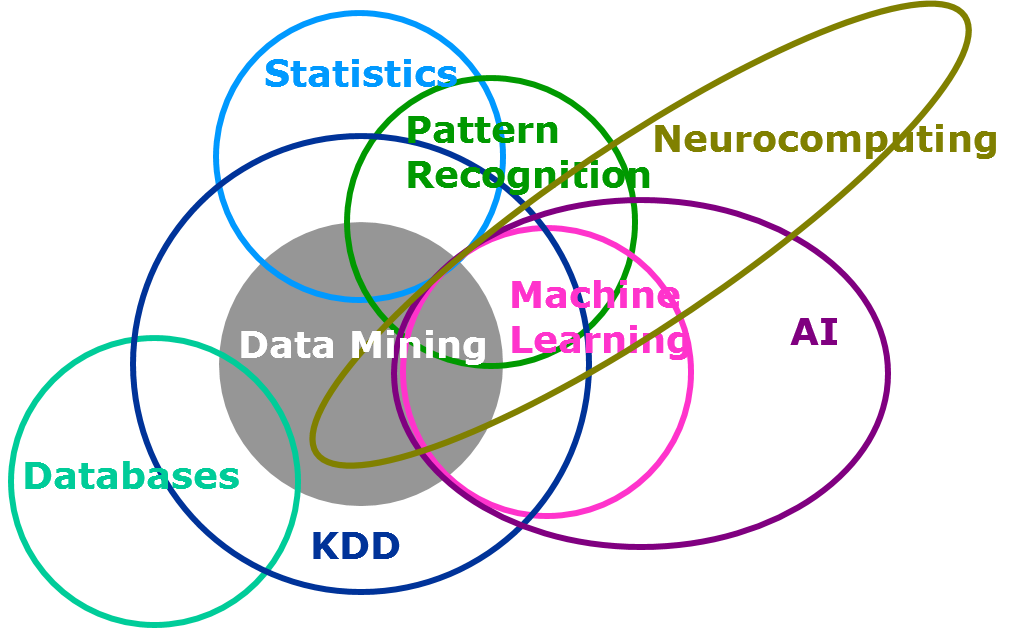
\includegraphics[width=10cm]{data-mining-Venn-diagram.png}
\centering
\caption{Machine Learninng as compared to other areas of data science.}
\label{fig:ML_comparison_image}
\end{figure}



%BACKGROUND
\section{Theory: Multiple Kernel Learning}

Multiple Kernel Learning (MKL) can be thought of as a tool, more than as an independent algorithm; it is an algorithm, but it is usually added to regression and classification algorithms, to improve their prediction power.

In a technical sense (see \cite{mehmet} for a more extense explanation of MKL), MKL can be defined as a set of machine learning methods that use a predefined set of kernels and learn an optimal linear or non-linear combination of kernels as part of the algorithm. In order to understand the somewhat cryptic previous sentence, MKL will be introduced here with very simple and commonly known tools.

\subsection{Support Vector Machines}

One way of solving the classification and regression problems, is using what is know as Support Vector Machines (SVM). SVM consists in that, given labeled training data, the algorithm outputs an optimal hyperplane which categorizes new examples. The rest of this subsection tries to explain the previous statement more clearly.

Imagine data as in figure \ref{fig:SVM_example1} (taken from \cite{svm_linear}), but now allowing a gap of size $\epsilon$ around the fitting line; in this case the SVM algorithm consists of a linear fitting, with the added property of summing the squares of distances only up to the dotted lines, and not up to the continuous (fitting) line. Once the algorithm is implemented, the data points which are on the dotted lines are called \textit{support vectors}, hence the name \textit{Support} Vector Machines.

\begin{figure}[t]
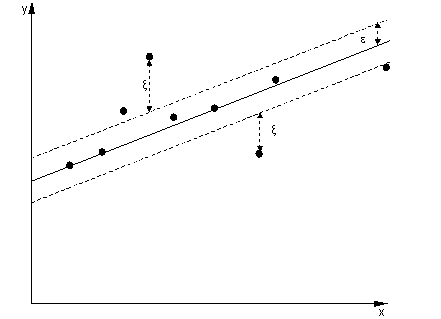
\includegraphics[width=11cm]{svm_exmpl}
\centering
\caption{SVM for linear regression.}
\label{fig:SVM_example1}
\end{figure}

The specific details of SVM are not important for understanding MKL, but there is a very important resultant property of the SVM algorithm:

\begin{center}
\textit{the evaluation of the relevant parameters of the model, depend exclusively on the dot products of the data}
\end{center}

More specifically (and to understand better the previous statement, but without going throught the whole SVM algorithm): if the dependent variable $y$ is to be modeled as a function of the independent variable $x$, and there are $n$ points of data, then, each of the $n$ points is characterised by a vector of the form $\vec{x}_{i} = \begin{pmatrix} x_{i} & y_{i}\end{pmatrix}$ (working in 2D here). Even more, the previous statement about dot products in SVM, means that the evaluation of the algorithm depends only on the elements in the following matrix (called the \textit{Kernel matrix}) $K$:

\begin{equation}
 X=\begin{bmatrix}
  \vec{x_{1}} \\
  \vec{x_{2}} \\
  ...\\
  \vec{x_{n}}
 \end{bmatrix} \rightarrow 
  K = XX^{T}
\label{eq:kernel_matrix}
\end{equation}

It is very important to understand that the dependance on only dot products, applies both to linear regression and linear classification, using SVM.


\subsection{From SVM to MKL}

There are algorithms, such as SVM which, when evaluating the data to find the parameters for the solution of the implementation, depend only on the values in $K$ (as introduced in equation \ref{eq:kernel_matrix}).

MKL is based on what is called \textit{the Kernel trick}. The Kernel trick is basically taking advantage of the feature mentioned before, that the evaluation of some algorithms depends only on dot products of the data.

\subsection{The Kernel trick}

If the available data is as in figure \ref{fig:MKL_example1}, it is clear that those points are not separable linearly. On the other hand, if the number of dimensions is expanded as in figure \ref{fig:MKL_example2}, then a hyperplane can be found, which separates data appropriately. The Kernel trick consists (partly) on performing such a change in dimensions.

\begin{figure}[t]
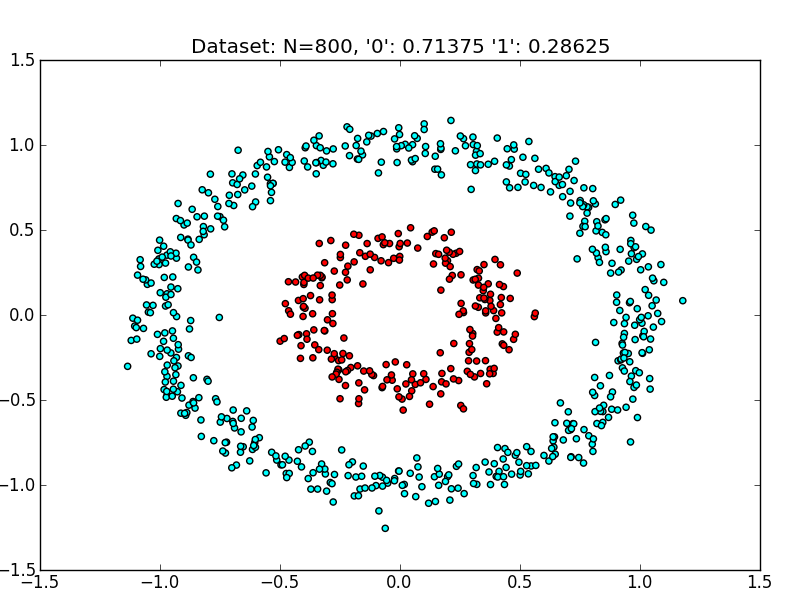
\includegraphics[width=11cm]{dataset_nonsep}
\centering
\caption{data not-linearly separable.}
\label{fig:MKL_example1}
\end{figure}

\begin{figure}[t]
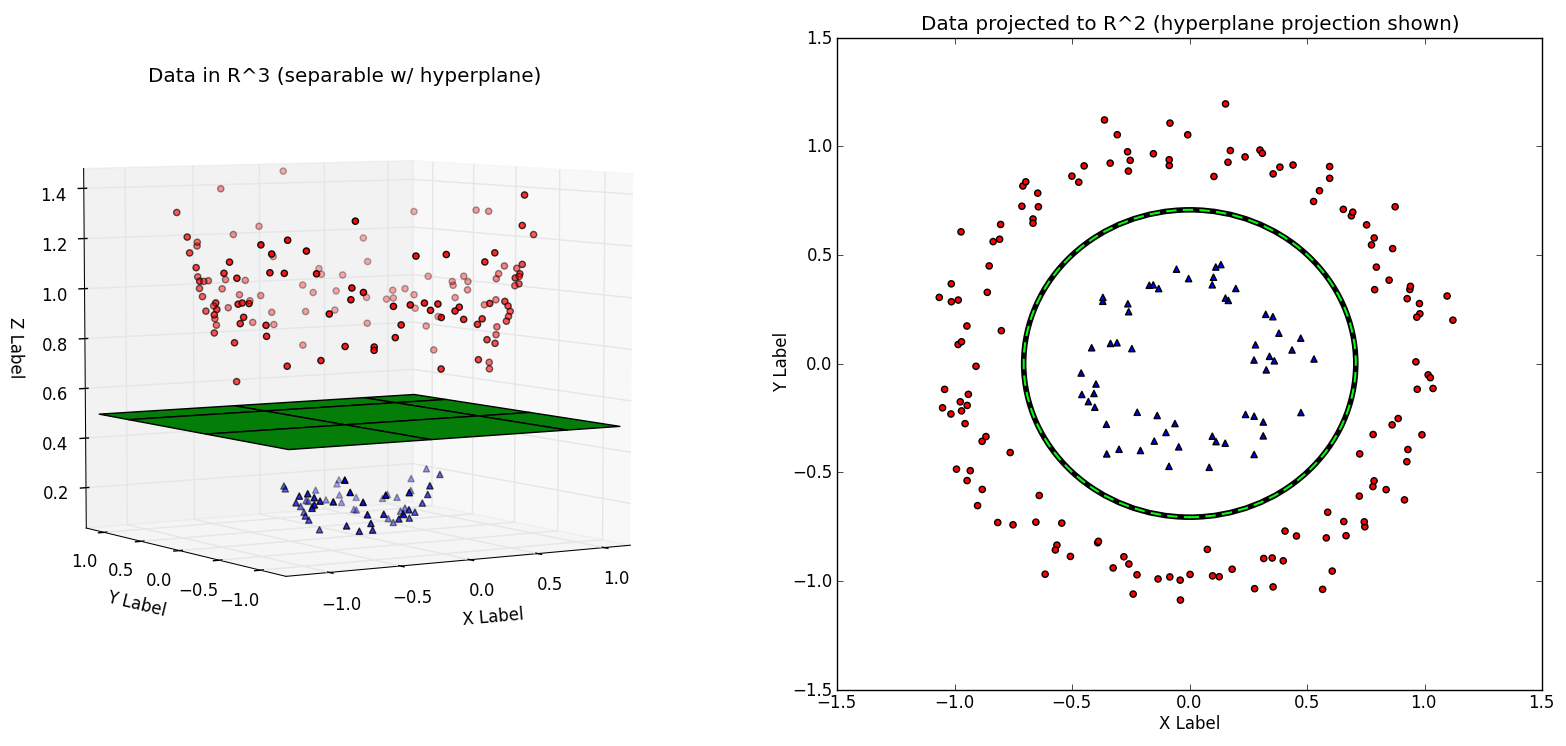
\includegraphics[width=15cm]{data_2d_to_3d_hyperplane}
\centering
\caption{separation of data throught the use of a dimensional change, through a hyperplane.}
\label{fig:MKL_example2}
\end{figure}

The other important feature of the Kernel trick comes from the form of the $K$ matrix. At this point, it is ideal to perform the dimensional change, in such a manner that the $K$ matrix keeps its form (why? Simply because the specific algorithm, SVM for example, can be reused if $K$ keeps its form), i.e. if the transformation is a function $\phi$ such that: $\phi: {\rm I\!R}^{2}\rightarrow {\rm I\!R}^{n}$, then, $K$ should have the form:

\[
K'=
  \begin{bmatrix}
    \phi(\vec{x_{1}})^{T}\phi(\vec{x_{1}}) & \phi(\vec{x_{1}})^{T}\phi(\vec{x_{2}}) & ...  \\
    \phi(\vec{x_{2}})^{T}\phi(\vec{x_{1}}) & ... & ...  \\
    ... & ... & ...
  \end{bmatrix}
\]

in such a manner that those dot producs (of the form $\phi(\vec{x_{i}})^{T}\phi(\vec{x_{j}})$) can be evaluated easily in terms of the dot products of the original $K$ matrix (i.e. terms of the form $\vec{x}_{i}\cdot \vec{x}_{j}$). In compact form, the Kernel trick consists in restricting the transformation $\phi$ by the following:

\begin{equation}
\phi(\vec{x_{i}})^{T}\phi(\vec{x_{j}}) = f(\vec{x}_{i}\cdot \vec{x}_{j})
\label{eq:kernel_matrix2}
\end{equation}


Here is a simple example on using the Kernel trick for an specific transformation from 2D to 3D:

\begin{itemize}
\item $\phi: {\rm I\!R}^{2}\rightarrow {\rm I\!R}^{3}$
\item transformation $\phi$: $(x_{1}, x_{2})\rightarrow (z_{1}, z_{2}, z_{3}) = (x_{1}^{2}, \sqrt{2}x_{1}x_{2}, x_{2}^{2})$
\item take ($\vec{r}$ and $\vec{s}$ are 3D, $\vec{a}$ and $\vec{b}$ are 2D): $\vec{r} = \phi(\vec{a})$ and $\vec{s} = \phi(\vec{b})$
\item $\Rightarrow (\vec{r}\cdot\vec{s})_{3D} = r_{1}s_{1}+r_{2}s_{2}+r_{3}s_{3} = (a_{1}^{2})(b_{1}^{2})+(\sqrt{2}a_{1}a_{2})(\sqrt{2}b_{1}b_{2})+(a_{2}^{2})(b_{2}^{2})$
\item $\Rightarrow (\vec{r}\cdot\vec{s})_{3D} = (\vec{a}\cdot\vec{b})^{2}$
\end{itemize}

and then, as shown, the dot products in 3D (after the transformation $\phi$ is taken) can be evaluated in terms of the dot products in 2D, only by squaring them.

As can be seen from the previous example and from equation \ref{eq:kernel_matrix2}, \textbf{no explicit knowledge of $\phi$ is necessary}, but the only thing that matters is the form of $f$. This is very powerful, as it allows to make use of extra dimensions, without having to compute the transformations driving the system towards the new dimensionally-extended form; but even more, it is very important, as there are functions $f(x)$ which lead to very complicated transformations $\phi(x)$, or even taking the system to an infinite dimensionality (i.e. $e^{\vec{x}\cdot \vec{y}}$).


\subsection{MKL}

The idea of MKL is making use of the Kernel trick, but now with a set of different functions: $\{ \phi_{1}, \phi_{2}, ..., \phi_{m} \}$.

Usually, in algorithms such as SVM, MKL can be easily plugged in. In simple SVM for linear regression, Lagrange multipliers are used for optimizing and reducing the error; this approach can be extended for integrating MKL into the mechanism, adding one extra Lagrange multiplier for each $\phi_{i}$ function.





%BENCHMARKING
%\section{Comparison with other methods.. when to use this?}

% - neural networks
 
% - others



%EXPLICIT FORM OF IMPLEMENTATION
\section{Applications}

Machine Learning is used in a lot of different areas (physics, biology, trading, etc.), solving a lot of different problems; the same goes for MKL, and specifically for the Kernel trick.

Extensions of MKL are frequently taken to solve complicated problems. For example, in reference \cite{cancer_research}, a study on cancer can be found, for which 44 different algorithms were used (and compared) in the prediction of sensitivity of cancer in response to the application of drugs; the algorithm which best performed was an extension of MKL using Bayesian Methods.




%CONCLUSIONS
\section{Conclusions}

\begin{itemize}
\item Multiple Kernel Learning is useful in algorithms such as SVM, where the evaluation of the parameters of the model makes use only of the dot products of the data vectors.
\item The Kernel trick consists in a dimensional extension from $d$ to $l$, for which the form of the Kernel matrix $K$ (containing the relevant information to solve the system) is preserved, and each element of that matrix is a function of the dot products in $d$-dimensions.
\item Each of the elements of the new matrix $K'$, after the transformation $\phi$ is taken, is simply the evaluation of the dot product in the original dimension, i.e. no explicit knowledge of $\phi$ is necessary.
\end{itemize}


%MATHEMATICAL DETAILS
%\section{Appendix}

%\subsection{Mathematical details of the Kernel Trick}


\newpage

%BIBLIOGRAPHY
%\section{References}

\begin{thebibliography}{1}

  \bibitem{bishop1} Christopher M. Bishop {\em Pattern Recognition and Machine Learning.}  2006: Springer.


  \bibitem{cancer_research} Costello \textit{et al.} {\em A community effort to assess and improve drug sensitivity prediction algorithms.} Nat Biotechnol. 2014 December; 32(12): 1202-1212.

  %\bibitem{impj}  The Japan Reader {\em Imperial Japan 1800-1945} 1973:
  %Random House, N.Y.

  \bibitem{mehmet} Mehmet G{\"o}nen and Ethem Alpaydin. {\em Multiple Kernel Learning Algorithms} 2011: Journal of Machine Learning Research 12.

  \bibitem{polly1} Polly Mitchell-Guthrie {\em Looking backwards, looking forwards: SAS, data mining, and machine learning} 2014: taken from: \\ http://blogs.sas.com/content/subconsciousmusings/2014/08/22/looking-backwards-looking-forwards-sas-data-mining-and-machine-learning/.

  \bibitem{svm_linear} {\em Support Vector Machine Regression} Taken from:
  http://kernelsvm.tripod.com/

  

  %\bibitem{fo} Bob Tadashi Wakabayashi {\em Anti-Foreignism and Western
  %Learning in Early-Modern Japan} 1986: Harvard University Press.

\end{thebibliography}




\end{document}